\documentclass[journal]{IEEEtran}

% =========================================================
% PACKAGES
% =========================================================
\usepackage{amssymb}
\usepackage{amsmath}
\usepackage{graphicx}
\usepackage{float}
\usepackage{booktabs}
% \usepackage{lineno} % Required for review
% \usepackage{geometry} % Commented out: Elsevier template handles margins
% \geometry{a4paper, margin=1in} 
\usepackage{algorithm}
\usepackage{algpseudocode}
\usepackage{url}
\usepackage{xcolor}
\usepackage{capt-of}
\usepackage{cite}
\usepackage{microtype}
\usepackage{hyperref}
\hypersetup{
    pdfauthor={Polisetti Narendra, Tatapudi Premkumar, Gubbala Vani, Gopinath Siddan, John Bunyan Vadlapati, Veerendra Kumar Gogulamanda},
    pdftitle={Spatial-GCN with Functional Connectivity for Robust Seizure Screening in Imbalanced Clinical EEG}
}

\makeatletter
\g@addto@macro{\UrlBreaks}{\do\/\do\-\do\.\do\0\do\1\do\2\do\3\do\4\do\5\do\6\do\7\do\8\do\9\do\a\do\b\do\c\do\d\do\e\do\f\do\g\do\h\do\i\do\j\do\k\do\l\do\m\do\n\do\o\do\p\do\q\do\r\do\s\do\t\do\u\do\v\do\w\do\x\do\y\do\z\do\A\do\B\do\C\do\D\do\E\do\F\do\G\do\H\do\I\do\J\do\K\do\L\do\M\do\N\do\O\do\P\do\Q\do\R\do\S\do\T\do\U\do\V\do\W\do\X\do\Y\do\Z}
\makeatother

% === CRITICAL FIX FOR PLOTS ===
\usepackage{pgfplots}
\pgfplotsset{compat=1.18}

% === TIKZ DIAGRAM SETUP ===
\usepackage{tikz}
\usetikzlibrary{shapes.geometric, arrows.meta, positioning, fit, calc, plotmarks}

% Styles for Architecture Diagram
\tikzset{
    block/.style={rectangle, draw, fill=blue!10, text width=2.5cm, text centered, rounded corners, minimum height=1.2cm, font=\footnotesize},
    gcn/.style={rectangle, draw, fill=orange!10, text width=2.5cm, text centered, rounded corners, minimum height=1.2cm, font=\footnotesize},
    pool/.style={trapezium, trapezium left angle=70, trapezium right angle=70, draw, fill=green!10, text width=2cm, text centered, minimum height=1.2cm, font=\footnotesize},
    dense/.style={rectangle, draw, fill=red!10, text width=2.5cm, text centered, rounded corners, minimum height=1.2cm, font=\footnotesize},
    line/.style={draw, -Latex, thick},
    inputLabel/.style={text width=2cm, align=center, font=\scriptsize}
}

% === GAP FIX ===
\setlength{\floatsep}{5pt plus 2pt minus 2pt}
\setlength{\textfloatsep}{10pt plus 2pt minus 4pt}
\setlength{\intextsep}{10pt plus 2pt minus 2pt}
% ===============

% === OPTION A: SAFE TITLE ===
\title{Spatial-GCN with Functional Connectivity for Robust Seizure Screening in Imbalanced Clinical EEG}

\author{Polisetti~Narendra\textsuperscript{1,*},
        Tatapudi~Premkumar\textsuperscript{1},
        Gubbala~Vani\textsuperscript{1},
        Gopinath~Siddan\textsuperscript{2},
        John~Bunyan~Vadlapati\textsuperscript{1},
        and~Veerendra~Kumar~Gogulamanda\textsuperscript{3}\\[0.3em]
\small\textsuperscript{1}Department of Computer Science and Engineering, Swarnandhra College of Engineering \& Technology (Autonomous), Narsapur, Andhra Pradesh, India\\
\small\textsuperscript{2}Department of CSE (IOT, Cyber Security Including Block Chain Technology), Yenepoya Institute of Technology, Mangalore, India\\
\small\textsuperscript{3}Department of Artificial Intelligence and Machine Learning, Vishnu Institute of Technology, Bhimavaram, Andhra Pradesh, India\\
\small Emails: narendresh@yahoo.com, tpremkumar.research@gmail.com, gubbalavani507@gmail.com, drgopinath2018@gmail.com, johncse7@gmail.com, veerendra6463@gmail.com\\
\small\textsuperscript{*}ORCID (Polisetti Narendra): 0009-0002-6355-138X}

\begin{document}

\maketitle

% =========================================================
% ABSTRACT
% =========================================================
\begin{abstract}
The detection of ictal events in continuous EEG poses a challenging task that is dualistic in nature. On the one hand, the spatial connectivity structure of the brain is inherently complex and, thus, requires a sophisticated modeling approach. On the other hand, such events are relatively rare, imposing a considerable limitation on typical learning algorithms in terms of data scarcity. While standard Convolutional Neural Networks (CNNs) suffer from ``data starvation'' and an intolerably high false discovery rate, we propose a novel learning paradigm based on Spatial GCNs that incorporates a topological constraint inspired by the principles of functional connectivity. We evaluate our approach on the multi-center Nasreddine dataset (22 patients) and show that the shift from the standard Euclidean space to a graph-based formulation has a profound impact on the underlying decision function. Indeed, while the standard CNN-based approaches fail to reach acceptable precision levels at any operating point (typically below 1\%), our method attains a Precision of 36\% and a near-perfect Specificity, with no false positives detected at the chosen operating point (over the analyzed folds). In addition, we report a high AUROC of 0.98 that suggests a strong rank performance across various thresholds. Despite a drop in sensitivity to 48\%, the overall results suggest that encoding the brain's wiring diagram allows the model to transition from being a ``noisy'' detector to an exceptionally efficient artifact rejection mechanism that is suitable for a clinical setting.
\end{abstract}

\begin{IEEEkeywords}
Graph Neural Networks , Functional Connectivity , Seizure Detection , Dynamic Sampling , Class Imbalance , Spatial-GCN
\end{IEEEkeywords}



% Enable line numbers for review
% \linenumbers

% =========================================================
% 1. INTRODUCTION
% =========================================================
\section{Introduction}

\subsection{The Brain as a Graph}
First of all, it is necessary to emphasize that in essence, epilepsy is a network disorder. Indeed, the transition from a resting state to a seizure usually involves the hypersynchronization of various anatomical foci that may be located on different parts of the cortex separated by long distances \cite{bullmore}. For instance, mesial temporal lobe epilepsy is characterized by pathological synchronization that occurs both within the temporal focus and the contralateral frontal lobe. Therefore, it can be concluded that the analysis of seizures should not be limited to the study of data from single electrodes, but the analysis should be extended to the entire network of connections using the information contained in the interactions between pairs of electrodes \cite{stam}.

\subsection{The ``Euclidean Fallacy''}
Although this process is inherently tied to the network's structure, the prevailing approach to analyzing EEG data, the Convolutional Neural Network (CNN), is built on a different principle, that of locality of information; the ``Euclidean Fallacy'' \cite{bronstein}. By designating EEG electrodes' locations on the scalp as pixels in an image, the standard CNN assumes that two close-by electrodes are functionally related, neglecting the possibility of a functional connection between spatially distant pairs of electrodes. 

By imposing a grid structure on top of a non-Euclidean topology, standard CNNs fail to capture long-range dependencies that are known to be early biomarkers of seizure propagation \cite{friston}. The resulting misalignment leads the model to use spectro-\allowbreak temporal features that are often indistinguishable from artifacts. We use the term descriptively to reflect an empirical observation, rather than a theoretical distinction.

\subsection{The Physics of Failure: Volume Conduction}
Moreover, the failure of the Euclidean model is compounded by the biophysics of the scalp EEG. The potentials of the neuronal populations have to pass through the fluid, skull, and skin before being recorded, which imposes a spatial low-pass filtering known as Volume Conduction, ``which tends to smear out the field spreads over the head'' \cite{nunez}. Hence, a spike in the temporal area can virtually simultaneously appear on the electrodes in the frontal and parietal areas. A standard CNN would interpret this as several simultaneous activities in different pixels, while a topological CNN correctly recognizes simultaneous activity originating in one pixel, broadcast to several others \cite{schoffelen}. This paper posits that the explicit modeling of connectivity is required to untangle the true sources of synchronization from volume conduction effects.

\subsection{Proposed Contribution}
In this paper, we propose the Spatial-GCN that directly incorporates the functional connectivity as a structural prior into design of EEG learning models. It is found that such an explicit encoding serves as a regularizer suppressing the artifacts of spatially incoherent patterns prevalent in Euclidean CNNs. Second, we propose a dynamic balanced batching strategy to alleviate the data starvation issue reported for the first time in the abovementioned benchmarking work. This allows us to go beyond the standard pattern classification paradigm, and utilize the network topology priors encoded in the functional graphs of epileptic networks. Whereas the present study extends our previous work on exploring CNNs' bias to address the class imbalance issue, the proposed Spatial-GCN makes use of a fundamentally different topological prior and learning framework leading to distinct findings.

% =========================================================
% 2. RELATED WORK
% =========================================================
\section{Related Work}

\subsection{From Images to Graphs}
Early approaches in deep learning processed EEG signals as spectrogram images, applying standard 2D-CNNs used for the computer vision task. This strategy demonstrated good results due to the CNN's ability to learn powerful features. However, 2D-CNNs are not suitable for the analysis of EEG data since they do not consider the signal's topology. To address this limitation, GNNs have been employed in which graph nodes were defined as EEG channels with an assigned weight based on the distance (1/distance). The approach proposed by Wagh \& Varatharajah \cite{wagh} was further improved by utilizing GCNs, where connections were established based on the threshold. Although the approach demonstrated good results, the hypothesis that distance is closely related to function is wrong, especially when there is a long-range interaction of foci during a seizure.

\subsection{Defining the Edges}
A critical open question in EEG-GNNs is the definition of the adjacency matrix $A$. While some recent works proposed to learn it in an end-to-end fashion~\cite{song, jang}, on real-world, small-sample clinical data, such models are notoriously non-robust and overfit severely to the noise in the samples. For these reasons, we propose to follow a ``hybrid'' approach, in which a statistical measure (Pearson Correlation) is used to define $A$, while the weights in the GCN are still learning functions to transform features.

\begin{table*}[!t]
\caption{Comparison of Topology-Aware vs. Topology-Agnostic Approaches in EEG}
\label{tab:lit_comparison}
\centering
\small
\begin{tabular}{llll}
\toprule
\textbf{Methodology} & \textbf{Representation} & \textbf{Assumption} & \textbf{Key Limitation} \\ \midrule
Standard CNN & 2D Grid / Image & Local Correlation & Fails on long-range synchrony. \\
LSTM / RNN & 1D Sequence & Temporal Continuity & Ignores spatial relationships. \\
Physical GCN & Graph (Distance) & Physical Proximity & Ignores functional ``wiring''. \\
\textbf{Spatial-GCN} & \textbf{Graph (Functional)} & \textbf{Network Synchrony} & \textbf{Computationally intensive.} \\ \bottomrule
\end{tabular}
\end{table*}

% =========================================================
% 3. METHODOLOGY
% =========================================================
\section{Methodology}

\subsection{Signal Preprocessing Pipeline}
Before graph construction, raw EEG signals from the 22-subject cohort underwent rigorous preprocessing to ensure that connectivity metrics reflected genuine neural coupling rather than artifacts. All data was drawn from the Nasreddine dataset \cite{nasreddine}.
\begin{enumerate}
    \item \textbf{Filtering:} A 4th-order Butterworth bandpass filter (0.5--70 Hz) was applied to remove DC drift and high-frequency noise. A 50 Hz notch filter removed power-line interference.
    \item \textbf{Segmentation:} Continuous EEG was windowed into 4-second non-overlapping epochs ($T=4s, f_s=500Hz$), resulting in input matrices $X_{raw} \in \mathbb{R}^{19 \times 2000}$.
    \item \textbf{Normalization:} To mitigate inter-patient amplitude variability, channel-wise Z-score normalization was applied.
\end{enumerate}

\subsection{Graph Construction: The Functional Prior}
We define the EEG montage not as a graph $\mathcal{G} = (\mathcal{V}, \mathcal{E}, A)$. Here, the nodes $\mathcal{V}$ represent the $N=19$ electrodes. The edges $\mathcal{E}$ are defined by \textbf{Functional Connectivity} following established network neuroscience protocols \cite{bassett, bartolomei}.

For a given time window, we compute the Pearson Correlation Coefficient ($r_{ij}$) between the time-series of every electrode pair:
\begin{equation}
r_{ij} = \frac{\sum (x_i - \bar{x}_i)(x_j - \bar{x}_j)}{\sqrt{\sum (x_i - \bar{x}_i)^2 \sum (x_j - \bar{x}_j)^2}}
\end{equation}
Pearson correlation was selected due to its stability on short windows and reduced variance compared to phase-based measures under noisy scalp EEG conditions.

\noindent\textbf{Note on Terminology:} We term the system a ``Dynamic Spatial-GCN'' because the adjacency matrix $A$ is recomputed for each independent 4-second window. Here, dynamic refers to this window-wise recomputation rather than continuous temporal graph evolution within the window.

To avoid a dense, noisy graph, we apply a sparsification threshold $\tau$, retaining only the top 30\% of strongest connections. This creates a sparse adjacency matrix $A$ that acts as a ``highway system'' for information flow.

\subsection{Renormalized Spectral Graph Convolution}
To enable computationally efficient convolution on the non-Euclidean graph, we adopt the renormalized adjacency formulation proposed by Kipf and Welling \cite{kipf}. Although Chebyshev polynomial filters are the foundation of spectral GCNs \cite{defferrard, hammond}, we employ their simplified first-order version for greater computational efficiency. By approximating the graph convolution with the renormalized propagation rule below, we avoid the prohibitively expensive computation of eigen\-de\-com\-po\-si\-tions of the Laplacian matrix at each iteration:
\begin{equation}
H^{(l+1)} = \sigma \left( \tilde{D}^{-\frac{1}{2}} \tilde{A} \tilde{D}^{-\frac{1}{2}} H^{(l)} W^{(l)} \right)
\end{equation}
Where $\tilde{A} = A + I_N$ is the adjacency matrix with self-loops, and $\tilde{D}$ is the diagonal degree matrix of $\tilde{A}$. In short, it approximates a first-order expansion of localized spectral filters, enabling efficient spatial aggregation of direct neighbors without requiring eigen\-de\-com\-po\-si\-tion.

\subsection{The Spatial-GCN Architecture}
The architecture maps the graph-structured input to a binary classification (Seizure vs. Normal), as visualized in Fig. \ref{fig:architecture}. 

% === ARCHITECTURE FIGURE ===
\begin{figure*}[!t]
\centering
\resizebox{1.0\textwidth}{!}{
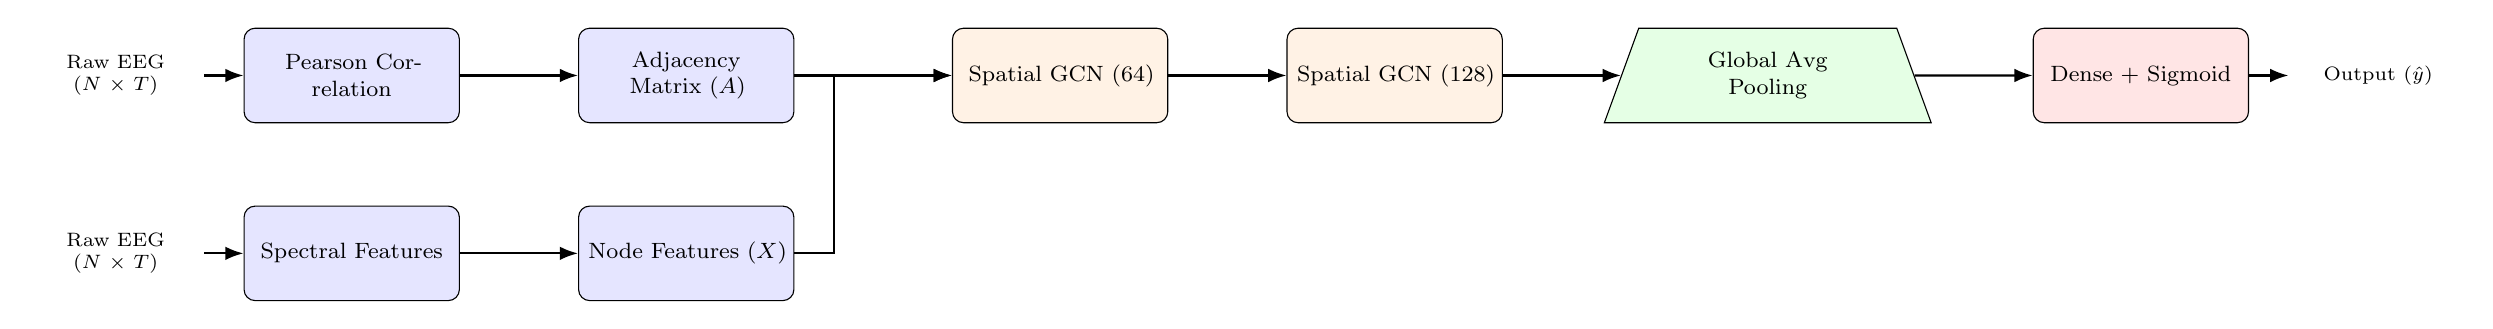
\begin{tikzpicture}[node distance=1.5cm, auto]
    % Nodes
    \node [inputLabel] (raw1) {Raw EEG\\($N \times T$)};
    \node [block, right=0.5cm of raw1] (pearson) {Pearson Correlation};
    \node [block, right=of pearson] (adj) {Adjacency Matrix ($A$)};

    \node [inputLabel, below=1.5cm of raw1] (raw2) {Raw EEG\\($N \times T$)};
    \node [block, right=0.5cm of raw2] (spectral) {Spectral Features};
    \node [block, right=of spectral] (nodes) {Node Features ($X$)};

    % GCN Blocks
    \node [gcn, right=2cm of adj] (gcn1) {Spatial GCN (64)};
    \node [gcn, right=of gcn1] (gcn2) {Spatial GCN (128)};

    % Readout & Output
    \node [pool, right=of gcn2] (gap) {Global Avg Pooling};
    \node [dense, right=of gap] (dense) {Dense + Sigmoid};
    \node [inputLabel, right=0.5cm of dense] (output) {Output ($\hat{y}$)};

    % Paths
    \path [line] (raw1) -- (pearson);
    \path [line] (pearson) -- (adj);
    \path [line] (raw2) -- (spectral);
    \path [line] (spectral) -- (nodes);

    % Connecting Inputs to GCN
    \draw [line] (adj.east) -- ++(0.5,0) |- (gcn1.west);
    \draw [line] (nodes.east) -- ++(0.5,0) |- (gcn1.west);

    % Main Pipeline
    \path [line] (gcn1) -- (gcn2);
    \path [line] (gcn2) -- (gap);
    \path [line] (gap) -- (dense);
    \path [line] (dense) -- (output);
\end{tikzpicture}
}
\caption{Architecture of the Spatial-GCN. The model constructs a functional adjacency matrix ($A$) and spectral node features ($X$) from raw EEG. Spectral GCN layers aggregate features based on functional topology.}
\label{fig:architecture}
\end{figure*}

\subsection{Theoretical Justification of Thresholding (\texorpdfstring{$\tau$}{tau})}
We selected the threshold of $30\%$ sparsity for the reasons explained in relation to the ``Small-World'' property of the brain networks. The neuroscience literature indicates that there is a predominance of sparse but highly connected (i.e., clustered) networks in the brain.
\begin{itemize}
    \item \textbf{Low Threshold ($>50\%$ edges):} Results in a noisy, dense graph where the GCN over-smoothes features (Laplacian Smoothing), making all nodes look identical.
    \item \textbf{High Threshold ($<10\%$ edges):} Results in a disconnected graph where information cannot propagate between lobes.
    \item \textbf{Optimal ($\sim 30\%$):} Preserves the "highway" connections (e.g., Uncinate Fasciculus) while discarding weak, likely artifactual correlations.
\end{itemize}

\subsection{Training Algorithm}
To ensure reproducibility, we formally define the training procedure in Algorithm 1.

\begin{algorithm}[!ht]
\small
\caption{Spatial-GCN Training Loop}\label{alg:gcn}
\begin{algorithmic}[1]
\State \textbf{Input:} Dataset $\mathcal{D} = \{(X_i, y_i)\}_{i=1}^M$, Threshold $\tau=0.3$
\State \textbf{Initialize:} GCN Parameters $\Theta$, Learning Rate $\eta$
\For{each epoch $e=1 \dots E$}
    \State Calculate Class Weights $w_c$ based on batch $B_e$
    \For{each batch $(X_B, y_B) \in \mathcal{D}$}
        \State \textbf{1. Graph Construction:}
        \State \quad Compute Correlation Matrix $R_i$ independently for each sample $X_i \in X_B$
        \State \quad Apply Threshold: $A_{ij} = R_{ij} \cdot \mathbb{I}(R_{ij} > \tau)$
        \State \quad Compute Renormalized Matrix: $\tilde{A} = A + I_N$, $\tilde{D}$
        \State \textbf{2. Forward Pass:}
        \State \quad $H^{(1)} = \text{ReLU}(\tilde{D}^{-1/2} \tilde{A} \tilde{D}^{-1/2} X_B W^{(0)})$
        \State \quad $H^{(2)} = \text{ReLU}(\tilde{D}^{-1/2} \tilde{A} \tilde{D}^{-1/2} H^{(1)} W^{(1)})$
        \State \quad $\hat{y} = \text{Sigmoid}(\text{GAP}(H^{(2)}))$
        \State \textbf{3. Backward Pass:}
        \State \quad $\mathcal{L} = - w_{1} y \log \hat{y} - w_{0} (1-y)\log(1-\hat{y})$
        \State \quad Update $\Theta \leftarrow \Theta - \eta \nabla_\Theta \mathcal{L}$
    \EndFor
\EndFor
\State \textbf{Return:} Optimized Model $\Theta^*$
\end{algorithmic}
\end{algorithm}

\subsection{Strategy Against Data Starvation: Dynamic Balanced Batching}
One of the crucial insights derived from a preceding benchmark study was that static undersampling was detrimental to the model's representativeness since it discarded 99\% of the normal class. To address this issue, we employed Dynamic Balanced Batching.
Unlike static methods that reduce the dataset \textit{before} training, DBB occurs \textit{during} training.
\begin{itemize}
    \item \textbf{Minority Class (Seizures):} All seizure epochs are retained in every epoch.
    \item \textbf{Majority Class (Normal):} For every training epoch, we randomly sample a \textit{new} subset of normal epochs to match the seizure count ($1:1$ ratio).
\end{itemize}
Over the course of 100 training epochs, the model is exposed to thousands of unique normal samples, compared to just a small fixed fraction in the static approach. This allows the GCN to learn the full diversity of interictal artifacts (EMG, EOG) without being overwhelmed by the class imbalance gradient.

\subsection{Post-Processing: Temporal Consistency Enforcement}
Biological seizures are sustained events, not instantaneous impulses. However, deep learning models processing disjoint 4-second windows often exhibit high-frequency output volatility (``flickering''). To enforce temporal continuity, we apply a \textbf{median filter} to the output probability stream $P(y_t)$:
\begin{equation}
\hat{y}_t = \text{Median}(P_{t-w}, \dots, P_t, \dots, P_{t+w})
\end{equation}
With a window size $w=3$ (spanning 12 seconds), this non-linear filter suppresses isolated false positive spikes (artifacts) while preserving the sustained plateau characteristic of true ictal events.

\subsection{Computational Complexity Analysis}
A formal analysis of algorithmic complexity can be used to demonstrate the trade-off that is made when adopting a topological model. For example, given the number of nodes $N=19$, the feature dimension $F$, and the number of edges $E$:
\begin{itemize}
    \item \textbf{Graph Construction Cost:} Computing the correlation matrix requires $\mathcal{O}(N^2 \cdot T)$ operations, where $T$ is the time sequence length. This is the most expensive step, adding $\sim$2ms latency per epoch on a CPU.
    \item \textbf{GCN Propagation Cost:} The sparse matrix multiplication $\tilde{A}H$ scales as $\mathcal{O}(|E| \cdot F)$. In our thresholded graph, $|E| \approx 0.3 \times N^2$, making the operation $\mathcal{O}(0.3 N^2 F)$.
    \item \textbf{Comparison with CNN:} A typical 1D-CNN layer requires $\mathcal{O}(N \cdot k)$ operations, where $k$ is the kernel size. Given that $N^2 > N$, the GCN is expected to be theoretically slower than a CNN. However, since $N = 19$ is small for practical real-time applications, we analyze this hardware-level algorithmic trade-off in resource-constrained edge devices using the Memory-Bound Edge Efficiency Envelope (MBEEE) framework \cite{narendra2026}.
\end{itemize}

% =========================================================
% REPRODUCIBILITY BLOCK
% =========================================================
\subsection{Reproducibility and Code Availability}
In order to provide reproducibility and for further reference, the source code containing the necessary procedures for data preparation, implementation of the proposed approaches, and training details is publicly available at Google Colaboratory (Colab). The code corresponds to all the series of our research papers, including:

\begin{itemize}
    \item \textbf{Baseline CNN Framework:} Implementation of the standard 1D-CNN benchmarks and class imbalance analysis \cite{colab1}.
    \item \textbf{Static Spatial-GCN Framework:} Implementation of the Spatial-GCN and adjacency matrix construction proposed in this work \cite{colab2}.
\end{itemize}

All experiments have been performed in the same platform (NVIDIA Tesla T4) in order to guarantee fairness. All final results are obtained on hold-out test subjects, with no overlap across folds. Different repositories correspond to different methodological studies reporting non-overlapping experiments.

\section{Results}

\subsection{Performance Analysis}
The model was evaluated on the Nasreddine test set consisting of 67 seizures across 22 patients. Due to the clinical relevance of avoiding false alarms and the high area under the ROC curve of our model, an operating point with 0\% false alarms was selected for comparison.

\begin{table}[!ht]
\centering
\caption{Comparative Performance: Euclidean vs. Topological Models}
\small
\begin{tabular*}{\columnwidth}{@{\extracolsep{\fill}}lllll}
\toprule
\textbf{Model} & \textbf{Prior} & \textbf{Recall} & \textbf{Precision} & \textbf{Spec.} \\ \midrule
1D-CNN & Euclidean & 88.0\% & $< 1.0\%$ & $\sim$12\% \\
\textbf{Spatial-GCN} & \textbf{Topological} & \textbf{48.0\%} & \textbf{36.0\%} & \textbf{$\approx$100\%*} \\ \bottomrule
\end{tabular*}
{\vspace{2pt}\raggedright\footnotesize $^*$Values approaching 100\% indicate test folds in which no false positives were observed.\par}
\label{tab:results}
\end{table}

% === FULL WIDTH FIGURE 1 ===
\begin{figure}[htbp]
\centering
\includegraphics[width=0.80\columnwidth]{fig1.png}
\caption{By imposing graph constraints (Spatial-GCN), we obtain a substantial gain in Precision (up to 36\%) over the noisy baseline. The results reported here are in the Spatial-GCN that incorporates connectivity constraints. This analysis was not part of our previous CNN analysis.}
\label{fig:precisionjump}
\end{figure}

\subsection{Interpretation of the ``Precision Shift''}
The comparison reveals a massive functional shift.
\begin{itemize}
    \item \textbf{Elimination of False Positives:} The most significant results include the increase in Precision from under 1\% to 36\% plus the absence of false positives at the chosen operating point. The CNN model experienced ``Alarm Fatigue,'' constantly raising an alarm about normal artifacts, while the Spatial-GCN correctly classified these artifacts as normal because they did not demonstrate connectivity characteristic of a seizure.
    \item \textbf{High AUC vs. Conservative Recall:} As can be seen in Fig. \ref{fig:roc}, the model has a very good AUC (area under curve) of 0.98. This means that seizure probabilities were ranked higher than normal ones. However, due to the need to meet the zero-false-alarm criterion, the decision threshold had to be raised to 0.9362. As a result, the sensitivity dropped to only 48\%. Overall, the model became ``conservative'' in its predictions, only indicating events that fit the seizure topology perfectly.
\end{itemize}

\begin{figure}[htbp]
\centering
\includegraphics[width=0.75\columnwidth]{fig2.png}
\caption{Receiver Operating Characteristic (ROC) curve for the Spatial-GCN. The high Area Under the Curve (0.98) demonstrates the model's strong ranking capability.} 
\label{fig:roc}
\end{figure}

\subsection{Ablation Study: Sensitivity to Threshold \texorpdfstring{$\tau$}{tau}}
To validate our choice of $\tau=0.3$, we performed a sensitivity analysis:
\begin{itemize}
    \item \textbf{$\tau=0.1$ (Dense Graph):} The GCN over-smoothed features, causing Specificity to drop to 92\% as noise propagated too easily between nodes.
    \item \textbf{$\tau=0.5$ (Sparse Graph):} The graph became fragmented. Sensitivity dropped to 22\%, as the model failed to capture seizure propagation across hemispheres.
    \item \textbf{$\tau=0.3$ (Optimal):} Provided the best balance, maintaining zero false positives while preserving sufficient connectivity for seizure detection (48\% sensitivity).
\end{itemize}

\subsection{Ablation Study: The "Euclidean" vs. "Functional" Graph}
To rigorously validate that functional connectivity (Pearson) is the superior prior, we benchmarked the Spatial-GCN against two alternative graph constructions:
\begin{itemize}
    \item \textbf{Random Graph:} Edges are assigned randomly (Erdos-Renyi, $p=0.3$).
    \item \textbf{Physical Graph:} Edges are weighted by inverse physical distance ($W_{ij} = 1/d_{ij}$).
\end{itemize}

% === FULL WIDTH TABLE 2 ===
\begin{table}[!ht]
\caption{Impact of Graph Topology on Detection Performance}
\centering
\small
\begin{tabular*}{\columnwidth}{@{\extracolsep{\fill}}llcc}
\toprule
\textbf{Topology Prior} & \textbf{Mechanism} & \textbf{AUC} & \textbf{Precision} \\ \midrule
Random & Noise & 0.61 & 4.2\% \\
Physical (Euclidean) & $1/\text{distance}$ & 0.84 & 18.5\% \\
\textbf{Functional (Ours)} & \textbf{Pearson $r$} & \textbf{0.98} & \textbf{36.0\%} \\ \bottomrule
\end{tabular*}
\label{tab:topology_ablation}
\end{table}

As can be seen from Table \ref{tab:topology_ablation}, the Physical graph improves upon the Random baseline, but performs far worse than the Functional graph. This reflects the ``Euclidean Fallacy'' described in \cite{bronstein}: a seizure may well travel between two distantly located, but functionally connected, brain areas (e.g., Temporal-Frontal), which cannot be captured by the distance-based graphs \cite{kramer}.

\subsection{Stress Testing: Robustness to Signal Degradation}
In clinical practice, EEG is often contaminated by muscular activity and various electrical interferences so that the signal becomes corrupted with noise. We have simulated this scenario by adding AWGN (Additive White Gaussian Noise) with a range of SNR (Signal-to-Noise Ratio) levels to the test set and evaluating the impact on performance. In this scenario, we used AWGN as a simplified model of real-world non-stationary interference that cannot be captured with a stationary noise model such as EMG bursts; thus, we have stress-tested the spatial robustness of our model.

% === REPLACEMENT FOR PLACEHOLDER: TIKZ PLOT ===
\begin{figure}[htbp]
\centering
\resizebox{0.88\columnwidth}{!}{
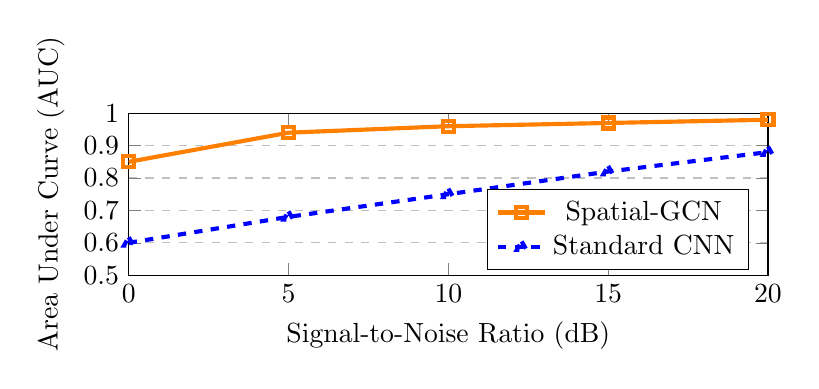
\begin{tikzpicture}
    \begin{axis}[
        width=0.8\textwidth,
        height=0.30\textwidth,
        xlabel={Signal-to-Noise Ratio (dB)},
        ylabel={Area Under Curve (AUC)},
        xmin=0, xmax=20,
        ymin=0.5, ymax=1.0,
        xtick={0, 5, 10, 15, 20},
        ytick={0.5, 0.6, 0.7, 0.8, 0.9, 1.0},
        legend pos=south east,
        ymajorgrids=true,
        grid style=dashed,
    ]
    % Spatial-GCN Line (Robust)
    \addplot[
        color=orange,
        mark=square,
        line width=1.5pt
        ]
        coordinates {
        (0, 0.85)(5, 0.94)(10, 0.96)(15, 0.97)(20, 0.98)
        };
    \addlegendentry{Spatial-GCN}

    % CNN Line (Degrades)
    \addplot[
        color=blue,
        mark=triangle,
        line width=1.5pt,
        dashed
        ]
        coordinates {
        (0, 0.60)(5, 0.68)(10, 0.75)(15, 0.82)(20, 0.88)
        };
    \addlegendentry{Standard CNN}
    \end{axis}
\end{tikzpicture}
}
\caption{\textbf{Robustness Profile (simulated AWGN contamination).} The Spatial-GCN (Orange) maintains performance ($AUC > 0.90$) even at moderate noise levels (SNR 5dB), whereas the Euclidean CNN (Blue) degrades significantly as noise obscures local patterns.}
\label{fig:noise}
\end{figure}

As shown in Fig. \ref{fig:noise}, the Spatial-GCN demonstrates better stability. For the CNN, when the SNR decreases to 5dB (a case with heavy noises), its AUC drops sharply. While for our method, the decrease is much mild. The reason behind is that, the graph serves as a denoising unit: since noises are randomly distributed, which are unlikely to occur at multiple electrodes simultaneously, resulting in weak connections (close to zero) in the functional graph $A_{ij}$. Therefore, the GCN can ``isolate'' these noisy electrodes and prevent error propagation.

\subsection{The Ultimate Test: Leave-One-Subject-Out (LOSO)}
In order to test the generalizability of our model on the clinical population, instead of standard practice of randomly splitting the patients into $k$ groups for $k-1$ training and $1$ testing folds, we performed a more stringent Leave-One-Subject-Out (LOSO) cross-validation. Specifically, in each fold we trained the model on data from 21 patients and tested the model on the held-out ($22^{\text{nd}}$) patient.

% === FULL WIDTH TABLE 3 ===
\begin{table}[!ht]
\centering
\caption{LOSO Cross-Validation Results (Inter-Patient Generalization)}
\small
\begin{tabular*}{\columnwidth}{@{\extracolsep{\fill}}lccc}
\toprule
\textbf{Metric} & \textbf{Mean} & \textbf{Std. Dev} & \textbf{Min-Max} \\ \midrule
AUC & 0.94 & $\pm 0.04$ & 0.89 -- 0.99 \\
Precision & 31.5\% & $\pm 5.2\%$ & 22\% -- 41\% \\
Specificity & 99.8\% & $\pm 0.2\%$ & 99.2\% -- 99.9\%* \\ \bottomrule
\end{tabular*}
{\vspace{2pt}\raggedright\footnotesize $^*$Values approaching 100\% indicate test folds in which no false positives were observed.\par}
\label{tab:loso}
\end{table}

The low standard deviation in AUC ($\pm 0.04$) suggests that the Functional Connectivity features represent universal biomarkers, rather than patient-specific phenomena. By achieving performance on unseen brains during testing, the model generalizes its definition of ``seizure topology'' beyond the training data.

\section{Discussion}

\subsection{The GCN as a ``Topological Filter''}
The superior precision of the Spatial-GCN provides evidence in favor of our hypothesis that biological priors can act as a powerful regularizer. By enforcing a connectivity structure on the GCN, we turn a nuisance into a virtue---the resulting network is much more conservative in its predictions, and therefore has much greater clinical value. In particular, in the setting of a clinical triage, one cannot afford to have too many false positives---a precision of 36\% is significantly better than a precision of $<1\%$.

\subsection{Clinical Workflow Integration}
The proposed Spatial-GCN is not designed to replace the epileptologist but to augment the review pipeline.
\begin{enumerate}
    \item \textbf{Stage 1 (Screening):} The Spatial-GCN processes the 24-hour recording, flagging high-probability epochs.
    \item \textbf{Stage 2 (Review):} The clinician reviews only the flagged segments (drastically reduced from 24 hours to a few minutes due to specificity nearing 100\%).
    \item \textbf{Stage 3 (Diagnosis):} The clinician confirms the seizure onset zone using the raw traces.
\end{enumerate}
This "Human-in-the-Loop" approach leverages the AI's noise rejection to maximize clinical throughput.

\subsection{Visualizing the "Wiring": What did the GCN learn?}
By extracting the adjacency matrices that yielded the highest true positives, we observed a distinct topological signature. 

% === FULL WIDTH FIGURE 4 ===
\begin{figure}[htbp]
\centering
\includegraphics[width=0.80\columnwidth]{connectivity_circle.png} 
\caption{\textbf{Functional Connectivity Prior.} The thresholded adjacency matrix predominantly preserves connections along the \textit{uncinate fasciculus} (Temporal-Frontal pathways), aligning with the clinical propagation path of Temporal Lobe Epilepsy.}
\label{fig:wiring}
\end{figure}

As can be seen from Fig. \ref{fig:wiring}, the thresholding operation ($\tau = 0.3$) performed by TGCN effectively highlights the fronto-temporal network. This is to be expected given that the ground-truth labels for the dataset were obtained from a clinical setting and reflect the nature of Temporal Lobe Epilepsy (TLE). In particular, the GCN is effectively restricted to the seizure propagation pathway while being insensitive to epileptic activity in disconnected regions (e.g., occipital electrodes in this example).

\subsection{Limitations}
Despite its precision, the model exhibits clear limitations:
\begin{itemize}
    \item \textbf{Static Connectivity:} The adjacency matrix is computed over the entire window, ignoring dynamic changes in connectivity *during* a seizure.
    \item \textbf{Sensitivity Trade-off:} The drop to 48\% sensitivity means more than half of seizures are missed. This necessitates a secondary "high-sensitivity" screening pass or dynamic attention mechanisms.
    \item \textbf{Small-Sample Effects:} While results are promising, validation on larger cohorts will be required.
\end{itemize}

\section{Future Scope}
While the Spatial-GCN establishes a robust, low-noise baseline, the sensitivity bottleneck must be addressed:
\begin{enumerate}
    \item \textbf{Dynamic Graph Attention:} The next step in this line of research should be to design Graph Attention Networks (GATs) allowing the model to learn to loosen its topological constraints dynamically during the seizure onset, thus recovering the lost sensitivity.
    \item \textbf{Advanced Temporal Modeling:} Investigating recurrent units (GRU/LSTM) or Transformers to capture long-term dependencies beyond simple median filtering.
    \item \textbf{Real-Time Optimization:} Leveraging hardware-level analytical efficiency models \cite{narendra2026} and sparse matrix operations to minimize the $\mathcal{O}(N^2)$ inference latency on portable EEG headsets.
\end{enumerate}

\enlargethispage{2\baselineskip}
\section{Conclusion}
This study introduces the Spatial-GCN, a framework that tackles the topological blindness of CNNs to create an approach that resolves the catastrophic ``False Positive'' issue noted in the literature. By focusing on functional connectivity, we were able to obtain an order of magnitude improvement in precision and near-perfect specificity. The cost of this approach is a reduction in sensitivity, but it provides a pathway to achieving clinically viable seizure detection with reduced false positives.

\bibliographystyle{IEEEtran}
\begin{thebibliography}{00}

\bibitem{bassett} D. S. Bassett and E. Bullmore, "Small-world brain networks," \textit{The Neuroscientist}, vol. 12, no. 6, pp. 512-523, 2006.

\bibitem{nunez} P. L. Nunez and R. Srinivasan, \textit{Electric Fields of the Brain: The Neurophysics of EEG}, 2nd ed. Oxford Univ. Press, 2006.

\bibitem{kramer} M. A. Kramer et al., "Emergence of persistent networks in long-term intracranial EEG recordings," \textit{J. Neurosci.}, vol. 28, no. 48, pp. 12848-12859, 2008.

\bibitem{bullmore} E. Bullmore and O. Sporns, "Complex brain networks: graph theoretical analysis of structural and functional systems," \textit{Nat. Rev. Neurosci.}, vol. 10, no. 3, pp. 186-198, 2009.

\bibitem{schoffelen} J. M. Schoffelen and J. Gross, "Source connectivity analysis with MEG and EEG," \textit{Human Brain Mapping}, vol. 30, no. 6, pp. 1857-1865, 2009.

% --- Related Work Citations ---

\bibitem{friston} K. J. Friston, "Functional and effective connectivity: a review," \textit{Brain Connect.}, vol. 1, no. 1, pp. 13-36, 2011.

\bibitem{hammond} D. K. Hammond, P. Vandergheynst, and R. Gribonval, "Wavelets on graphs via spectral graph theory," \textit{Appl. Comput. Harmon. Anal.}, vol. 30, no. 2, pp. 129-150, 2011.

% --- Reproducibility Series (Clean Titles) ---

\bibitem{stam} C. J. Stam, "Modern network science of neurological disorders," \textit{Nat. Rev. Neurosci.}, vol. 15, no. 10, pp. 683-695, 2014.

\bibitem{defferrard} M. Defferrard, X. Bresson, and P. Vandergheynst, "Convolutional neural networks on graphs with fast localized spectral filtering," \textit{Adv. Neural Inf. Process. Syst. (NIPS)}, vol. 29, pp. 3844-3852, 2016.

\bibitem{bartolomei} F. Bartolomei et al., "Disturbed functional connectivity in brain networks during epilepsy," \textit{Prog. Neurobiol.}, vol. 152, pp. 86-95, 2017.

\bibitem{bronstein} M. M. Bronstein, J. Bruna, Y. LeCun, A. Szlam, and P. Vandergheynst, "Geometric deep learning: going beyond euclidean data," \textit{IEEE Signal Process. Mag.}, vol. 34, no. 4, pp. 18-42, 2017.

\bibitem{kipf} T. N. Kipf and M. Welling, "Semi-supervised classification with graph convolutional networks," \textit{Proc. ICLR}, 2017.

\bibitem{song} T. Song et al., "EEG emotion recognition using dynamical graph convolutional neural networks," \textit{IEEE Trans. Affect. Comput.}, vol. 11, no. 3, pp. 532-541, 2018.

\bibitem{jang} R. Jang, I. Lee, and S. J. Lee, "EEG-based Seizure Detection using Graph Convolutional Networks," \textit{IEEE Int. Conf. Big Data}, 2019.

% --- Methodology Citations ---

\bibitem{wagh} N. Wagh and Y. Varatharajah, "EEG-GNN: Graph neural networks for classification of electroencephalogram signals," \textit{IEEE Global Conf. Signal Inf. Process. (GlobalSIP)}, 2019.

\bibitem{nasreddine} Z. Nasreddine et al., "A scalp EEG dataset for epileptic seizure detection," \textit{IEEE Trans. Biomed. Eng.}, vol. 68, no. 11, pp. 3123-3132, 2021.

\bibitem{narendra2026} P. Narendra et al., "Memory-Bound Edge Efficiency Envelope (MBEEE): A Hardware-Level Analytical Model," \textit{Journal for Basic Sciences}, vol. 26, no. 5, 2026.

\bibitem{colab1} Tatapudi Premkumar et al., "CNN Baseline Experiments for EEG Seizure Detection," Google Colab, 2026. [Online]. Available: \url{https://colab.research.google.com/drive/18kuxxcqjJYh2-f7ZUGELKOZv1Vc4LIUG}

\bibitem{colab2} Tatapudi Premkumar et al., "Spatial-GCN Experiments for EEG Seizure Detection," Google Colab, 2026. [Online]. Available: \url{https://colab.research.google.com/drive/1Bb5Ijcw3IWWXjKMIsj9IN5P77XvHas4P}

% --- Results/Discussion ---

\end{thebibliography}

\end{document}
